\documentclass[letterpaper,11pt]{article}
\usepackage{amsmath}
\usepackage{moreverb}
\usepackage{amssymb}
\usepackage{graphicx}
\usepackage{mathtools}
\usepackage{tikz}
\usepackage{pgfplots}
\usepackage{float}
\usetikzlibrary{arrows,shapes, positioning}
\DeclarePairedDelimiter\floor{\lfloor}{\rfloor}
\let\biconditional\leftrightarrow
\addtolength{\oddsidemargin}{-.875in}
\addtolength{\evensidemargin}{-.875in}
\addtolength{\textwidth}{1.75in}
\addtolength{\topmargin}{-.875in}
\addtolength{\textheight}{1.75in}
\newenvironment{customlegend}[1][]{%
    \begingroup
    % inits/clears the lists (which might be populated from previous
    % axes):
    \csname pgfplots@init@cleared@structures\endcsname
    \pgfplotsset{#1}%
}{%
    % draws the legend:
    \csname pgfplots@createlegend\endcsname
    \endgroup
}%

% makes \addlegendimage available (typically only available within an
% axis environment):
\def\addlegendimage{\csname pgfplots@addlegendimage\endcsname}

\pgfkeys{/pgfplots/number in legend/.style={%
        /pgfplots/legend image code/.code={%
            \node at (0.295,-0.0225){#1};
        },%
    },
}

\title{Distributed Systems -- Term Project}
\author{Jacob Errington (260636023) \\ Alexandre Laporte (260635979)}
\date{3 December 2015}

\begin{document}

\maketitle

\section{Design and architecture}

Our distributed system consists of eight logical components.

\begin{enumerate}
    \item
        The \emph{Middleware Layer} is the core component of the system. It is
        in turn connected to many other components and acts as a coordinator
        for all messages. It is in particular equipped with a
        \emph{Transaction Manager} and it is connected to many
        \emph{Resource Managers}.

    \item
        The \emph{Transaction Manager} tracks transactions on a global level
        and maintains information about the overall state of the transactions
        in the system.
        The \emph{Transaction Manager} also keeps track of which
        \emph{Resource Managers} are involved in which transactions.

    \item
        The \emph{Client} makes requests to the \emph{Middleware}.

    \item
        For each type of data to be stored in the system, there is one
        \emph{Resource Manager}. Each resource manager tracks the transactions
        with which is it involved, and to each transaction, it associates a
        \emph{Persistence Layer}, \emph{Lock Manager} and \emph{Datastore}.

    \item
        The \emph{Persistence Layer} is used to persist data to disk in a
        reliable way.

    \item
        The \emph{Lock Manager} implements a two-phase locking scheme to ensure
        safe accesses to data items stored in the \emph{Datastore}.

    \item
        The \emph{Datastore} is a synchronized in-memory hashtable equipped
        with serialization support for interaction with the
        \emph{Persistence Layer}.

    \item
        The \emph{Network Layer} is used to proxy calls to methods of remote
        objects over reliable TCP sockets.
\end{enumerate}

The system stores four main types of data: flights, cars, rooms, and customers.
The system is also able to record reservations of flights, cars, and rooms by
customers.

We distribute this data across four nodes, one for each main type of data. The
node tracking a particular type of reservable items also holds information
about the reservations on that item.

For simple requests, the middleware dispatches the request to the backend
server corresponding to the type of request. Once the backend server's reply is
received, it is transmitted back to the client.

More complex requests such as reservations require additional work from the
middleware server. For example, in order to reserve a flight, the middleware
must first ensure that the customer exists by querying the customer server,
and then reserves the flight by sending a request to the flight server. The
case of printing a bill is even more complicated as it requires querying every
backend server once.

\begin{figure}[H]
    \centering

    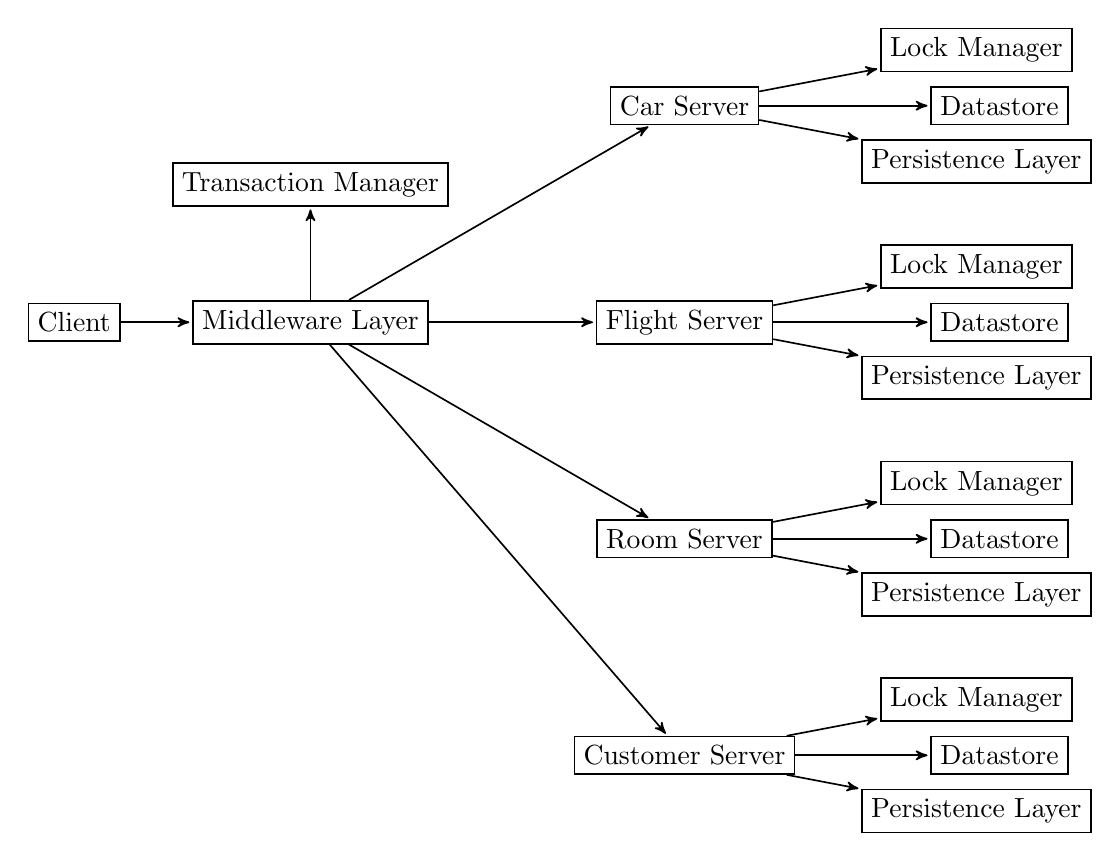
\begin{tikzpicture}[->,>=stealth',shorten >=1pt,auto,node distance=1cm,semithick]
        \node[draw] (rect) (client) 
            {Client};

        \node[draw] (rect) (middleware) [right of=client,xshift=2cm]
            {Middleware Layer};

        \node[draw] (rect) (TM) [above of=middleware, node distance=1.75cm]
            {Transaction Manager};

        \node[draw] (rect) (flight) [right of=middleware,xshift=3.75cm]
            {Flight Server};

        \node[draw] (rect) (car) [above of=flight, yshift=1.75cm]
            {Car Server};

        \node[draw] (rect) (room) [below of=flight, yshift=-1.75cm]
            {Room Server};

        \node[draw] (rect) (customer) [below of=room, yshift=-1.75cm]
            {Customer Server};

        \node[draw] (rect) (flightDB) [right of=flight, xshift=3cm]
            {Datastore};

        \node[draw] (rect) (carDB) [right of=car, xshift=3cm]
            {Datastore};

        \node[draw] (rect) (roomDB) [right of=room, xshift=3cm]
            {Datastore};

        \node[draw] (rect) (customerDB) [right of=customer, xshift=3cm]
            {Datastore};

        \node[draw] (rect) (flightLM) [above right of=flight, xshift=3cm]
            {Lock Manager};

        \node[draw] (rect) (carLM) [above right of=car, xshift=3cm]
            {Lock Manager};

        \node[draw] (rect) (roomLM) [above right of=room, xshift=3cm]
            {Lock Manager};

        \node[draw] (rect) (customerLM) [above right of=customer, xshift=3cm]
            {Lock Manager};

        \node[draw] (rect) (flightPL) [below right of=flight, xshift=3cm]
            {Persistence Layer};

        \node[draw] (rect) (carPL) [below right of=car, xshift=3cm]
            {Persistence Layer};

        \node[draw] (rect) (roomPL) [below right of=room, xshift=3cm]
            {Persistence Layer};

        \node[draw] (rect) (customerPL) [below right of=customer, xshift=3cm]
            {Persistence Layer};

        \path
        (client)     edge                node {} (middleware)
        (middleware) edge                node {} (TM)
        (middleware) edge                node {} (flight)
                     edge                node {} (car)
                     edge                node {} (room)
                     edge		         node {} (customer)
        (flight)     edge                node {} (flightDB)
        (car)        edge                node {} (carDB)
        (room)       edge                node {} (roomDB)
        (customer)   edge 		         node {} (customerDB)
        (flight)     edge                node {} (flightLM)
        (car)        edge                node {} (carLM)
        (room)       edge                node {} (roomLM)
        (customer)   edge 		         node {} (customerLM)
        (flight)     edge                node {} (flightPL)
        (car)        edge                node {} (carPL)
        (room)       edge                node {} (roomPL)
        (customer)   edge 		         node {} (customerPL)
        ;
    \end{tikzpicture}

    \caption{
        The architecture of our system uses a middleware server to contact
        independent backend servers to perform tasks related to different types
        of reservable items. Each backend server uses in-memory synchronized
        hashtables to store their respective data. Furthermore, each backend
        server is equipped with a lock manager, enabling it to perform strict
        two-phase locking; a persistence layer, enabling it to safely persist
        data to disk; and a lock manager to ensure that accesses to data items
        do not violate transaction isolation. Since each backend server has its
        own datastore, data consistency \emph{between} backend servers is
        maintained by the middleware. The middleware generates random
        identifiers for transactions as they are created.
    }
\end{figure}

At the core of both the middleware and backend servers, there is a tight loop
that accepts incoming connections. Upon each new connection being established,
a handler is created for that connection and is run in a different thread. We
use a pool with a fixed number of threads based on the number of logical
processors on the machine. Consequently, new connections may be accepted while
requests are being handled in these worker threads, and many requests may be
processed concurrently.

Objects are sent over the network using Java's built-in serialization
capabilities. However, we pass only two types of objects over the network.

\begin{description}
    \item[Request.] A request object represents a remote method invocation on
        the recipient server's ResourceManager. As such, it simply contains the
        name of the method to invoke, an array of objects to use as parameters,
        and some metadata on the parameters. The request object implements a
        method using reflection to invoke the method on a provided object
        implementing the resource manager interface. This allows us to remain
        agnostic about the precise implementation of this interface, and
        consequently, we can use identical request objects for both
        client-middleware and middleware-backend communications.

    \item[Response.] A response object represents the return value of the
        remote method invocation. Since remote method invocations may abruptly
        fail, we bracket the method calls with exception handlers that
        package the exception into the response object and return it to the
        client, where it is thrown again. This allows exceptions to
        transparently be thrown across the network, and prevents exceptions
        raised by event handler code from crashing the socket accept loop.
        However, clients and the middleware must take care to check for these
        exceptions as they are unchecked.
\end{description}

\begin{figure}[H]
    \centering

    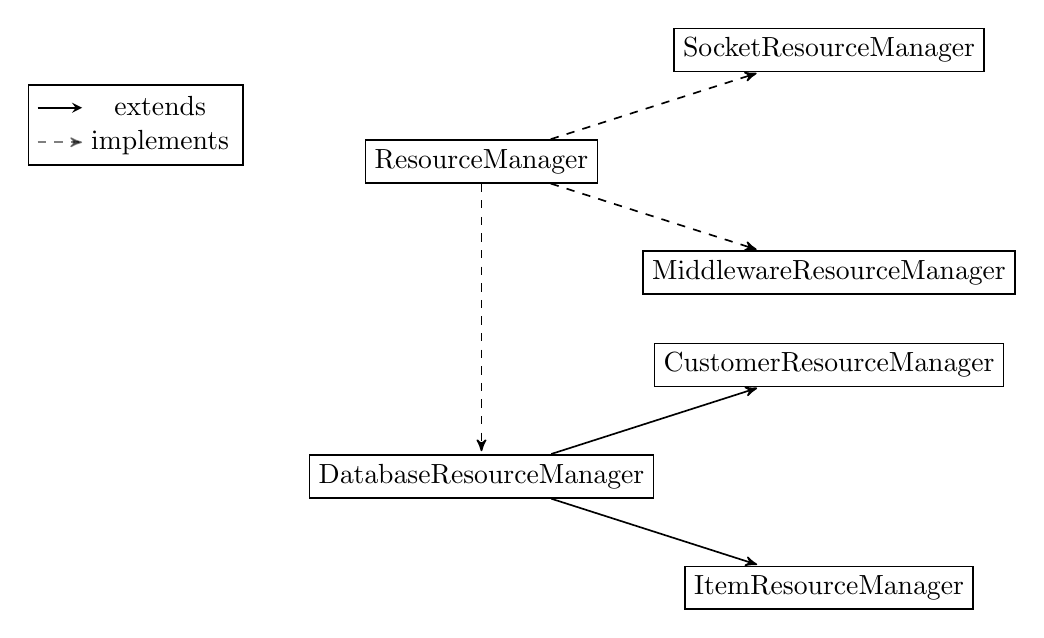
\begin{tikzpicture}[->,>=stealth',shorten >=1pt,auto,node distance=2cm,semithick]
        \node[draw] (rect) (RM) [xshift=4cm] {ResourceManager};
        \node[draw] (rect) (SRM) [above right of=RM, xshift=3.0cm] {SocketResourceManager};
        \node[draw] (rect) (MRM) [below right of=RM, xshift=3.0cm] {MiddlewareResourceManager};
        \node[draw] (rect) (DRM) [below of=RM, node distance=4.0cm] {DatabaseResourceManager};
        \node[draw] (rect) (CRM) [above right of=DRM, xshift=3.0cm] {CustomerResourceManager};
        \node[draw] (rect) (IRM) [below right of=DRM, xshift=3.0cm] {ItemResourceManager};
        \path
        (RM) edge[dashed] node {} (SRM)
             edge[dashed] node {} (MRM)
             edge[dashed] node {} (DRM)
        (DRM) edge node {} (CRM)
              edge node {} (IRM)
        ;

        \begin{customlegend}[
            legend entries={ % <= in the following there are the entries
                extends,
                implements
            }
        ] % <= to define position and font legend
          % the following are the "images" and numbers in the legend
            \addlegendimage{-stealth,black,opacity=1}
            \addlegendimage{black,dashed,opacity=0.5}
        \end{customlegend}
    \end{tikzpicture}

    \caption{
        The inheritance structure of our main classes is shown above.
        Each component of the system is represented by a class implementing the
        \texttt{ResourceManager} interface, which defines the basic set of
        capabilities that can be performed on reservable items.
        Backend servers use a \texttt{CustomerResourceManager} or a
        \texttt{ItemResourceManager} to perform actions on their respective
        backing store,  according to the type of data that they manage.
        Since many operations are the same in both cases, we introduce the
        \texttt{DatabaseResourceManager} superclass, which includes facilities
        to persist data to disk securely.
        Clients use a \texttt{SocketResourceManager} to send \texttt{Request}
        objects representing the remote methods to call.
        The middleware server's \texttt{MiddlewareResourceManager} aggregates a
        number of \texttt{SocketResourceManager}s, one for each connected
        backend server. Many requests received by the middleware simply need
        to be forwarded to the appropriate backend server, but some requests
        require aggregating data across all nodes in order to present summary
        information to the client.
    }
\end{figure}

\section{Performance of distributed transactions}

Below we show the performance of distributed transactions in the system.
Figure \ref{fig:performance-vs-tps} shows the performance of the system under
concurrent loads, whereas figure \ref{fig:throughput} presents an evaluation of
the throughput of the system.

\begin{figure}[ht]
    \centering
    \includegraphics[width=0.8\textwidth]{figure.pdf}
    \caption{
        Requests are submitted by ten clients concurrently at an
        increasing rate. The performance of the system as the rate of
        transactions being submitted increases degrades as expected in a
        slightly sublinear fashion.
    }
    \label{fig:performance-vs-tps}
\end{figure}

\begin{figure}[ht]
    \centering
    \includegraphics[width=0.8\textwidth]{bars.pdf}
    \caption{
        A single client bombards the system with requests in order to evaluate
        the overall throughput of the system according to the complexity of the
        submitted requests. Requests involving one, two, and three independent
        backend servers are submitted. Despite the varying complexity of these
        requests, the difference in average response times are not significant.
    }
    \label{fig:throughput}
\end{figure}

\section{Data model and persistence scheme}

Our data model is very simple. Data to be transferred over the network is
packaged into \texttt{Request} and \texttt{Response} objects as described in
the general architecture section.

At the datastore level, the data naturally arranges itself into maps: flights
are keyed on their flight number, and cars and rooms are keyed on their
location. We call the set of all reservable items under a given key an
\emph{ItemGroup}. Each ItemGroup has a count of the total number of items, map
describing reservations on the items, a computed count of reserved items, a
price, and a description of the type of item. The main data record is merely a
map from keys to ItemGroups. We call this map a \emph{Data} record. It suffices
to persist this map to disk when a transaction completes.

When a ResourceManager is enlisted in a transaction, it sets up its own
initally empty Data record. When queries, inserts, or updates are performed in
the context of the transaction, the ResourceManager will use the LockManager
associated with the transaction to obtain the appropriate lock on the record
being accessed, and it will copy the affected record from the main Data to the
transaction-local Data. Hence, no writes are directly made to the main Data.

When a ResourceManager receives a vote request from the Middleware, it marks
the transaction as internally having progressed to the \texttt{PREPARED} state,
persists the transaction-local Data to disk, and persists the list of
\texttt{PREPARED} transactions to disk before sending its vote to the
Middleware. If the ResourceManager fails before receiving the decision from the
Middleware, it will load the list of \texttt{PREPARED} transactions from disk.
(It is stored in a predictable location.) From this list, it computes the
location of the persisted transaction-local Data for each \texttt{PREPARED}
transaction, load the transaction-local Data from disk, and query the
Middleware to determine the fate of the transaction. Three answers are
possible.
\begin{itemize}
    \item
        The transaction is still in the \texttt{PREPARED} state.
        This means that the 2PC protocol is still in phase one. The
        ResourceManager simply adds the transaction-local Data that it loaded
        to its list of \texttt{PREPARED} transactions and starts up as normal.
        It receives the decision from the Middleware later.

    \item
        The transaction has entered the \texttt{COMMITTED} state.
        This means that all participants voted \texttt{YES}. The
        ResourceManager can run its Data merging routine to incorporate the
        changes from the transaction-local Data to the main Data.

    \item
        The transaction has entered the \texttt{ABORTED} state.
        This means that at least one participant voted \texttt{NO}. The
        transaction-local Data that was loaded from disk may simply be
        discarded.
\end{itemize}

If we allow the possibility of the Middleware failing, one more answer is
possible: the transaction is in the \texttt{UNKNOWN} state, i.e. the Middleware
does not know about the transaction whose status is being queried by the
ResourceManager. Indeed, we did not implement a recovery procedure at the
Middleware level. If the Middleware fails, all global state regarding the
transaction is lost. In this case, we assume at the ResourceManager level that
the transaction was aborted and discard the transaction-level Data.

Furthermore, because the Middleware loses all its state if it fails, it loses
track of which transaction identifiers are in use. A scheme of incremental
transaction identifiers is unsatisfactory due to the following scenario.

The Client starts a transaction. The Middleware assigns the next available
identifier to the transaction; it assigns the number $0$. The Client performs
an operation that enlists ResourceManager $m$. The Middleware then fails. The
Client performs an operation involving transaction $0$, but this operation
fails because the Middleware is now unaware of any transaction $0$ existing.
The Client then starts a new transaction. The Middleware na\"ively assigns
the number $0$ to this next transaction. The Client performs another operation
involving ResourceManager $m$. This in turn will cause that ResourceManager to
be enlisted a second time.

Now we are left with a dilemma. Either the ResourceManager throws an exception
if it is enlisted a second time, indicating to the Middleware that it should
abort transaction $0$ and forcing the Client to call \texttt{start} again to
get the next transaction identifier, or the ResourceManager silently allows
itself to be enlisted a second time, sneakily bringing any changes that were
made before into this new transaction $0$.

Neither of these situations provides behaviour that would not be considered
astonishing. Instead, we simply use a scheme of assigning \emph{random} numeric
identifiers to transaction. This makes it very unlikely that the same
transaction identifier will be assigned more than once before the transaction
times out at each site.

\section{Challenges}

Different challenges were faces in different stages of the development of this
system.

\begin{description}
    \item[Deliverable \#1.]
        In the first deliverable, the main challenge was in the use of SOAP.
        Our team is significantly more well-versed in the concepts of REST,
        which require much less instrumentation of build scripts and such.

        Furthermore, we chose to make our lives somewhat unnecessarily
        difficult by replacing the existing hashtable data structures with
        Postgres. In fact, we initially misunderstood the assignment
        instructions and centralized all the data in a single database. We then
        needed to quickly rework the codebase to use four separate databases.
        This proved to be quite difficult in the time frame that we had.

    \item[Deliverable \#2.]
        In the next deliverable, in which we needed to develop distributed
        transactions, we realized that sticking with Postgres wouldn't work.
        We were unable to figure out how to use Postgres as a backing store for
        our own transaction system without resorting to using Postgres's
        built-in transaction support, which would defeat the purpose of the
        assignment.

        We entirely pivoted our codebase to use distributed hashtables. Again
        however, we chose to make our lives difficult. (Who doesn't like a
        challenge?) Rather than use the provided hashtables from deliverable
        \#1, we implemented our own from scratch. Likewise, rather than use the
        provided LockManager, we created a different lock management system on
        our own terms. This allowed it to more easily integrate with our
        existing codebase.

    \item[Deliverable \#3.]
        By this point, the codebase is over six thousand lines of Java,
        scattered among some sixty files. Following the chains of method calls
        that collectively accomplish something is now rather difficult, and
        analyzing the potential for concurrency errors is even harder.

        This may be due to a lack of foresight on our part in the development
        of the prior deliverables, but on the other hand, it is rather hard to
        properly architect the codebase when it is not yet known what the
        requirements of the future deliverables is.
\end{description}

\section{Testing}

Our testing scheme involved adding new methods to the interactive client to
allow us to simulate failures.

First, we created a SimulatedFailureManager singleton class holding a single
variable of an enumerated type whose values represent the different types of
failures we want to simulate. Then, in relevant locations in the code, we check
what the value of this variable is to determine whether to crash or not.
Crashing is accomplished by exiting with a nonzero exit code. Sometimes we
wanted to crash \emph{after} sending a reply. Our networking layer is so
general however that it would have been extremely difficult to modify it to
inspect the response it is sending in order to crash precisely after the
response is sent. Instead, we use a \texttt{ScheduledExecutorService} to have a
thread run one second after we return from the request handler, which should be
enough time for the reply to be transmitted.

In order to automate recovery, we then instrumented the execution of each
program with a bash script to automatically restart the program until it exits
with a nonzero exit code.

The overall effect is that the client can set a global failure mode, causing
crashes in predictable ways which will automatically recover after. The client
console can then perform some more introspection to verify that the system is
left in a consistent state.

\end{document}
